%%%%%%%%%%%%%%%%%%%%%%%%%%%%%%%%%%%%%%%%%%%%%%%%%%%%%%%%%%%%%%%%%%%%%%%%%%%%%
%	e-Yantra, IIT-Bombay

%	Document Author: Saurav Shandilya
%	Date: 16-August,2012
%	Last Editted by: Saurav
%   Date Last updated: 31-05-2016 

%%%%%%%%%%%%%%%%%%%%%%%%%%%%%%%%%%%%%%%%%%%%%%%%%%%%%%%%%%%%%%%%%%%%%%%%%%%%%

\documentclass[11pt,a4paper]{article}
\usepackage{graphicx}
\usepackage{caption}
\usepackage{hyperref}
\usepackage{graphicx}
\title{Interfacing GPS with APM}
\author{Akshit Gandhi \\ Keyur Rakholiya}
\date{June 16, 2016}

\begin{document}
	\maketitle
	\newpage
	\tableofcontents
	\newpage
	\section{Tutorial Name}
	Interfacing GPS with APM
	\section{Prerequisites}
	Before reading this tutorial read about APM and read DATASHEET of your GPS module.
	\section{Hardware Requirement}
	\begin{center}
	\includegraphics[width=200px]{gps}
		\captionof{figure}{GPS}
	
	
	\includegraphics[width=200px]{ardu}
		\captionof{figure}{APM 2.6 FLIGHT CONTROLLER}
	\end{center}
	\newpage
	\section{Software Requirement}

	MISSION PLANNER SOFTWARE 1.3.30

	\section{Theory and Description}
		connect the GPS to APM via GPS port which is given in APM.
		follow this image for connections.
		\begin{center}

		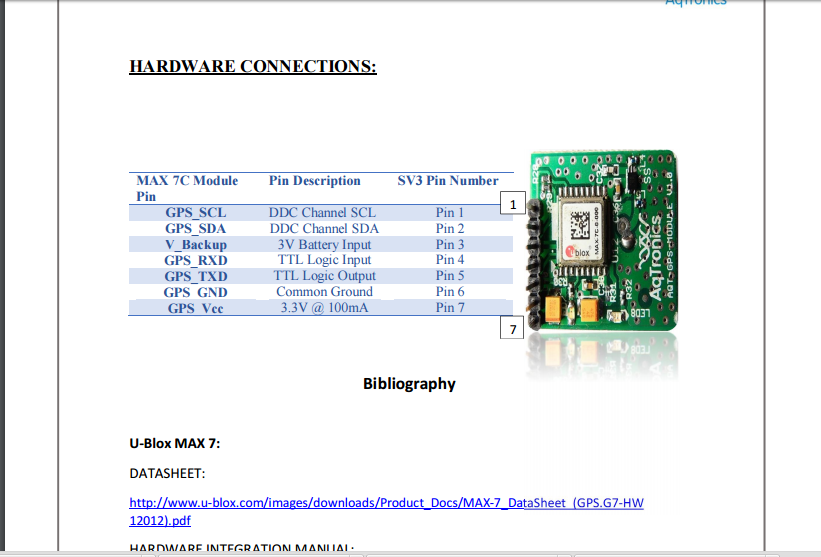
\includegraphics[width = 300px]{gps2}
			\captionof{figure}{GPS module pin Diagram}
		
		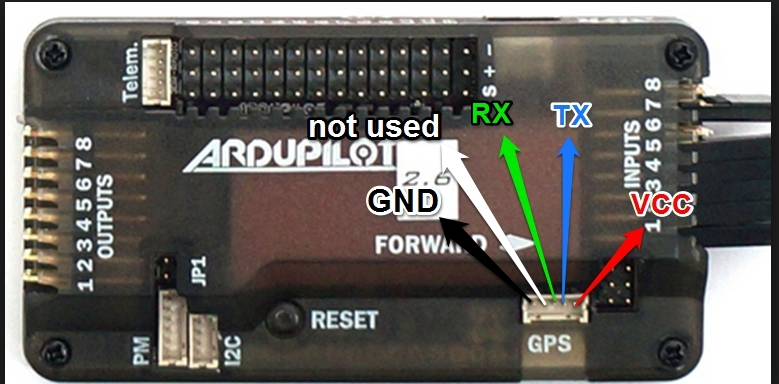
\includegraphics[width = 300px]{ardu2}
			\captionof{figure}{GPS Pin on APM}
		\end{center}
		
		\vspace{1in}
		connect the module as shown in figure. connect APM with Mission planner and go to under open sky.
		for perfect gps location you GPS module should be under open sky. after 2 or 3 minutes GPS satellites will be connected to module. and you will find your Location on map in MISSION PLANNER software. you can also see no. of satellites connected to your gps module. \\
		
		you will also get value of longitude,latitude,altitude on terminal of mission planner software.\newline
		
		\begin{center}
		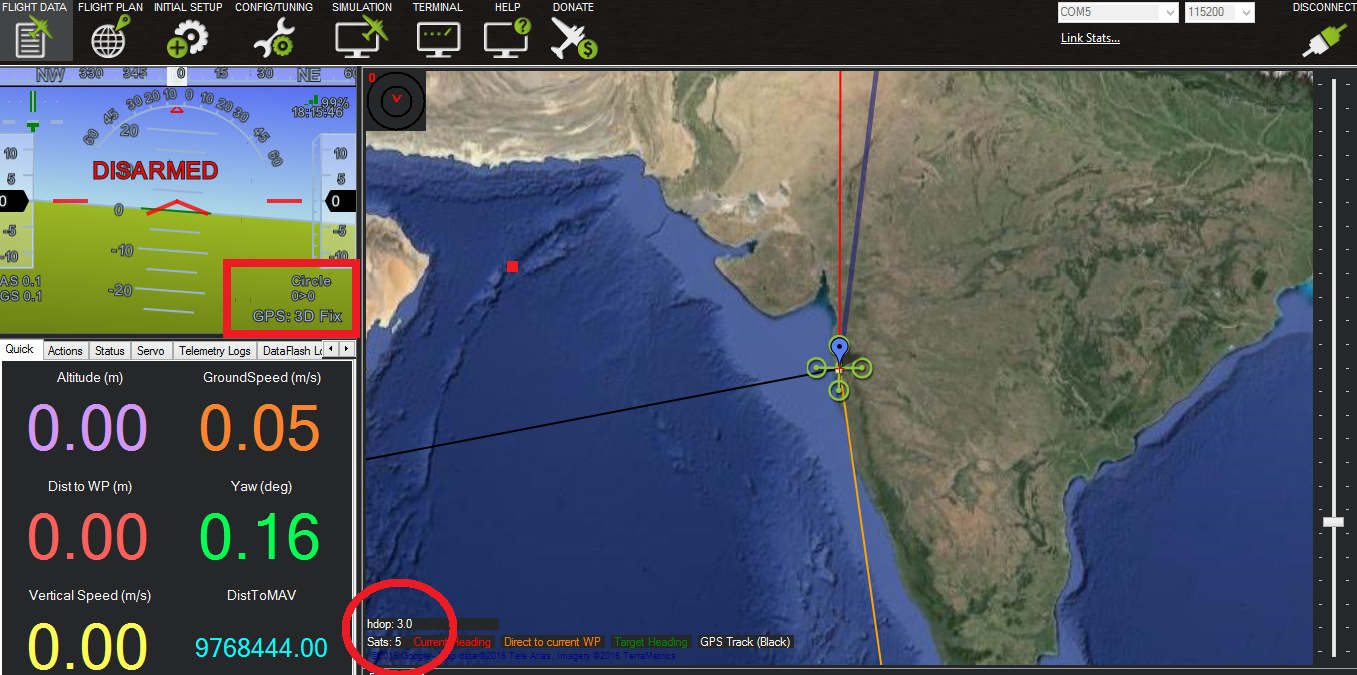
\includegraphics[width = 400px]{map1}
		\captionof{figure}{current location}
		\end{center}
		\hspace{0.5in}
		as you can see in the figure. mission planner shows 3D fix and no. of satellites are 5.
		
		\newpage
		\hspace{0.5in}
		as you move from one place to another you will be tracked as you can see in image.
			\begin{center}
				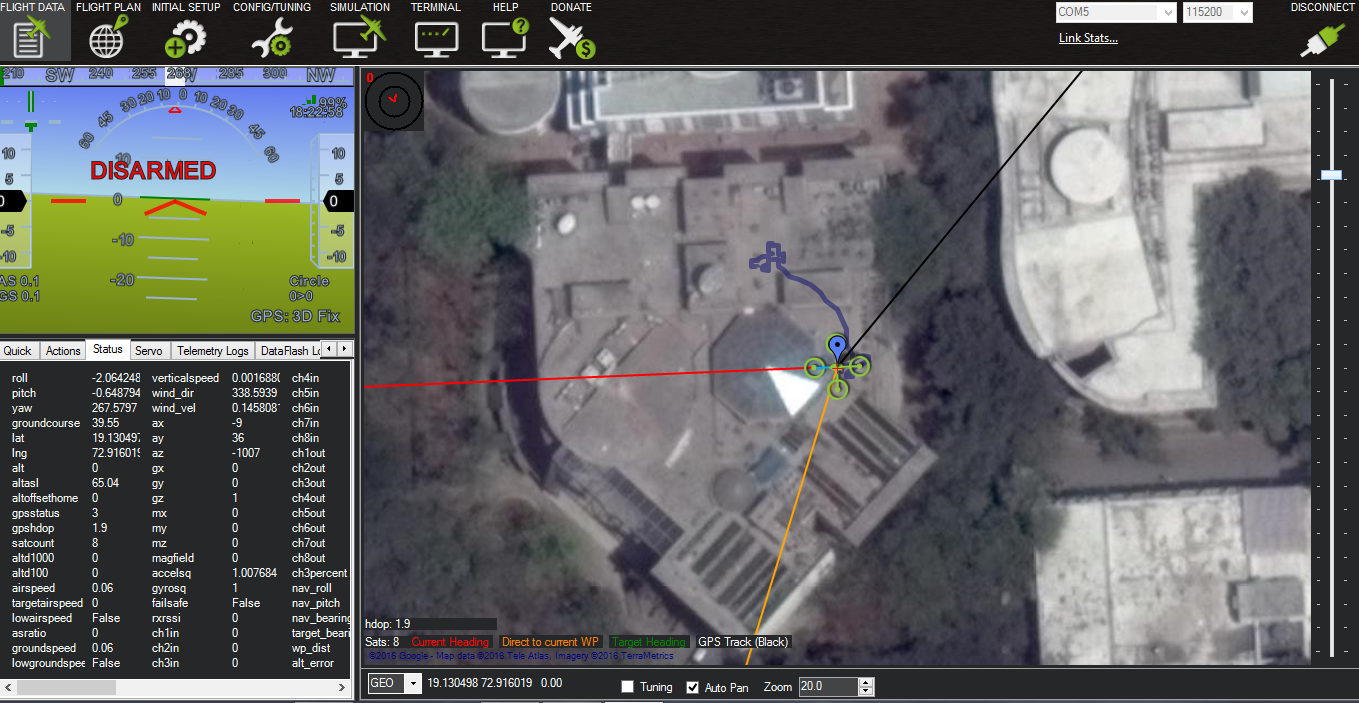
\includegraphics[width = 400px]{map2}
				\captionof{figure}{closer look to location}
			\end{center}
	you can see  LAT , LON ,ALT and SATS on terminal.
		\begin{center}
			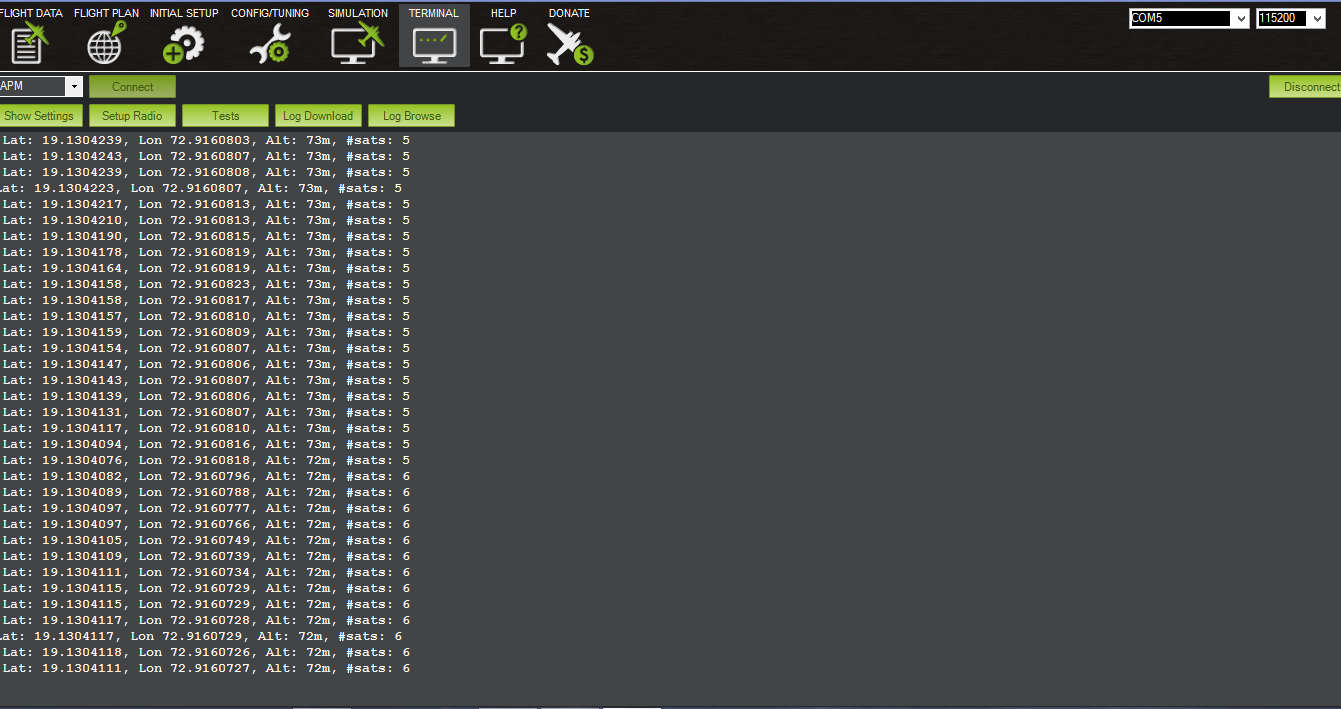
\includegraphics[width = 400px]{map3}
			\captionof{figure}{DATA from terminal}
		\end{center}

	\section{References}
	\url{http://ardupilot.org/copter/docs/common-installing-3dr-ublox-gps-compass-module.html}
	\paragraph{•}
		 Our GPS datasheet.
\end{document}



